The toolchain follows the methodology described in \sref{methodology}. It
consists of a number of command-line tools, and the tools are composed of a
number of stand-alone packages. We also make use of third-party software,
including the simulators introduced in \sref{literature}. The toolchain is
publicly available online at \cite{sources}.

The main programs of the toolchain are called \emph{Recorder} and
\emph{Streamer}, which we discuss in the following subsections.

\subsection{Recorder} \slab{recorder}
\begin{figure}
  \centering
  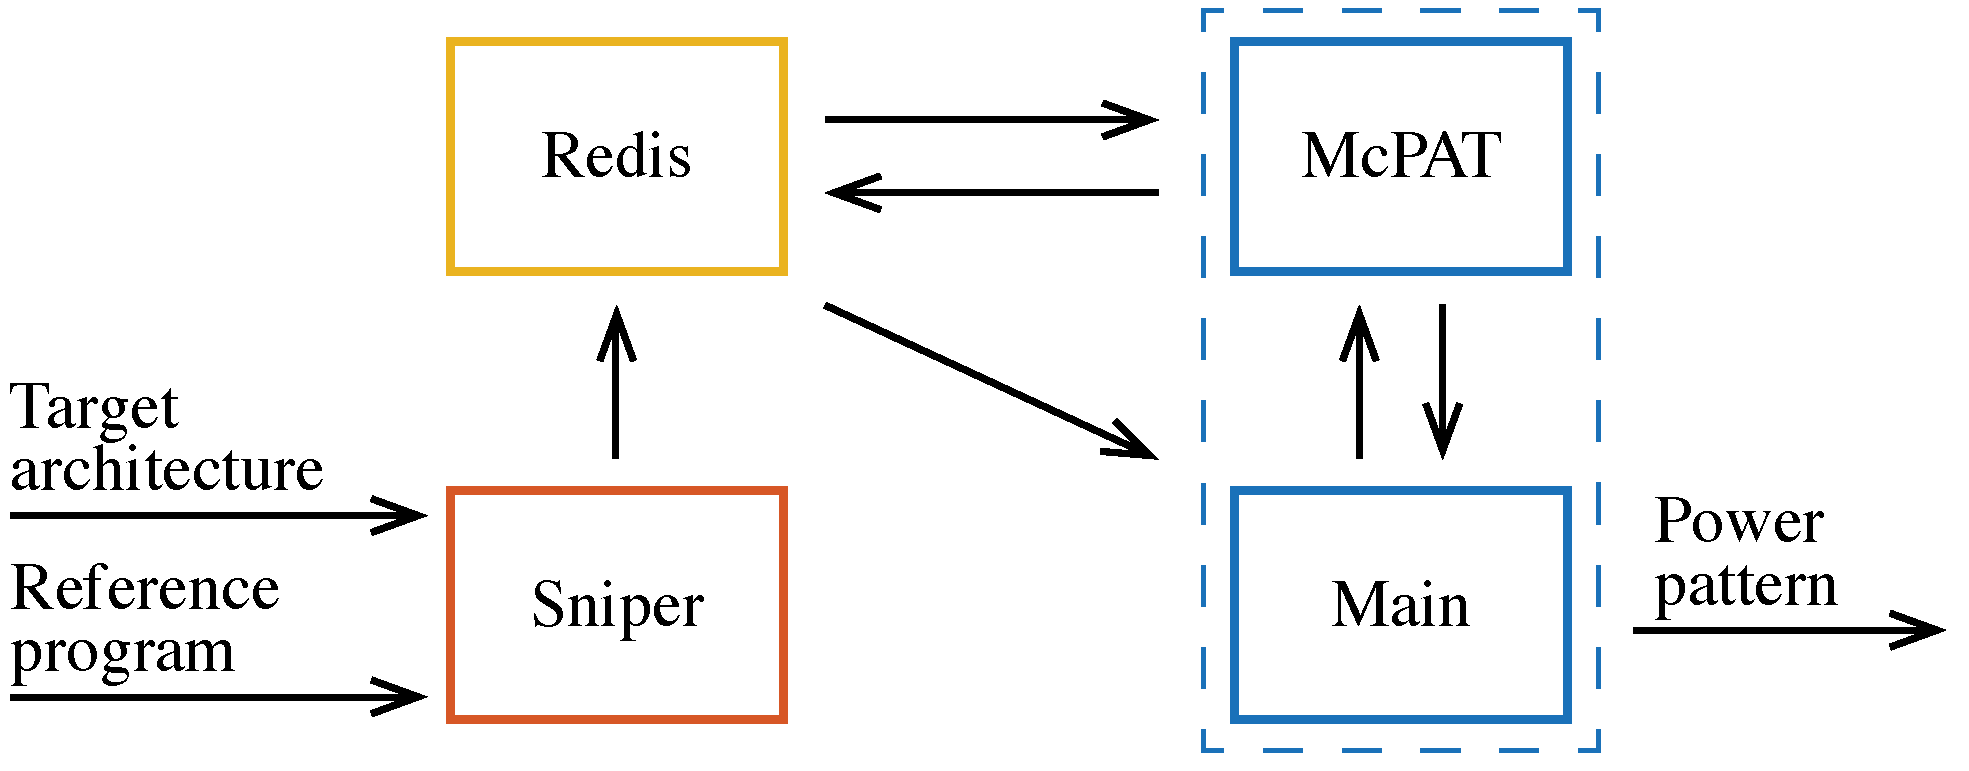
\includegraphics[width=1.0\columnwidth]{include/assets/figures/recorder.pdf}
  \caption{The recording infrastructure.}
  \flab{recorder}
\end{figure}

As the name suggests, the purpose of \recorder\ is recording. More specifically,
the tool records power traces, which are needed as an input to \streamer. The
recording infrastructure is depicted in \fref{recorder}.

Sniper \cite{carlson2011}.
\begin{table}
  \caption{Target architecture}
  \begin{tabular*}{\linewidth}{=L{70pt}l}
    \toprule
    Component    & Description \\
    \midrule
    Core         & 2660 MHz, 1.2 V \\
    L1-I/D cache & 32 KB, 4-way, LRU, private \\
    L2 cache     & 256 KB, 4-way, LRU, private \\
    L3 cache     & 8192 KB, 16-way, LRU, one per four cores \\
    \bottomrule
  \end{tabular*}
  \tlab{target}
\end{table}
% vim: nowrap tw=0


The key-value storage is Redis \cite{redis}. The database is SQLite
\cite{sqlite}.

\sc{McPAT} \cite{li2009}.


\subsection{Streamer} \slab{streamer}
\begin{figure}
  \centering
  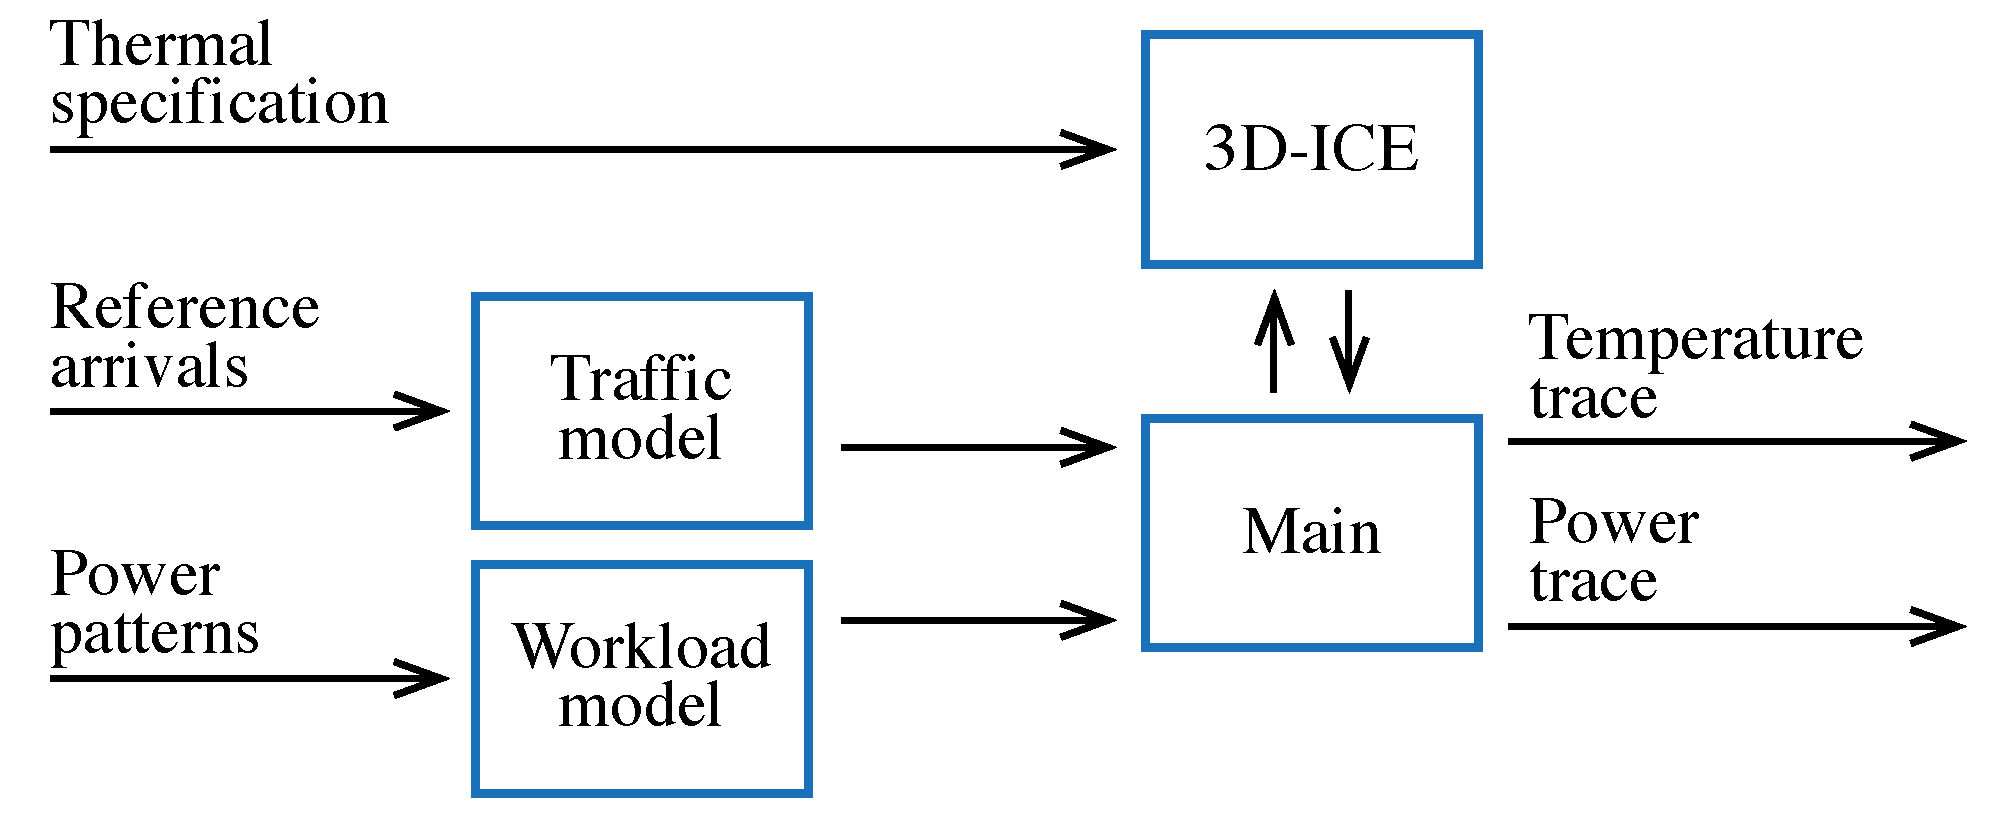
\includegraphics[width=1.0\columnwidth]{include/assets/figures/streamer.pdf}
  \caption{The streaming infrastructure.}
  \flab{streamer}
\end{figure}

The streaming infrastructure is depicted in \fref{streamer}.

HotSpot \cite{skadron2004}.
\sc{3D-ICE} \cite{sridhar2010}.
The solver is based on exponential integrators \cite{hochbruck2010},
\cite{ukhov2012}.

